% Adjust these for the path of the theme and its graphics, relative to this file
%\usepackage{beamerthemeFalmouthGamesAcademy}
\usepackage{../../beamerthemeFalmouthGamesAcademy}
\usepackage{multimedia}
\graphicspath{ {../../} }

% Default language for code listings
\lstset{language=C++,
        morekeywords={each,in,nullptr}
}

% For strikethrough effect
\usepackage[normalem]{ulem}
\usepackage{wasysym}
\usepackage{gensymb}
\usepackage{pdfpages}
\usepackage{verbatim}


% http://www.texample.net/tikz/examples/state-machine/
\usetikzlibrary{arrows,automata}

\newcommand{\modulecode}{COMP260}\newcommand{\moduletitle}{Distributed Systems}\newcommand{\sessionnumber}{5}

\begin{document}
\title{\sessionnumber: Expert Evaluation}
\subtitle{\modulecode: \moduletitle}

\frame{\titlepage} 

\begin{frame}
	\frametitle{Sign the Register}
	\begin{figure}
		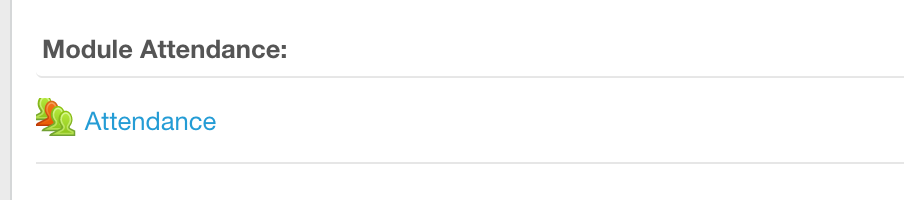
\includegraphics[scale=.5]{assets/attendance}
		\caption{\tiny{http://learningspace.falmouth.ac.uk/course/view.php?id=1254\&section=1 }}
	\end{figure}
\end{frame}

\begin{frame}
	\frametitle{Learning Outcomes}
	After this session you will be able to:

	\begin{itemize}
		\item \textbf{Describe} the difference between expert, automated \& user testing.
		\item \textbf{Justify} the choice of heuristics for various situations
		\item \textbf{Implement} a heuristic evaluation.
	\end{itemize}
\end{frame}

\begin{frame}
	\frametitle{Types of Usability Testing}
	
	According to Lazar et al., there are three different types of usability testing:

	\begin{itemize}
		\item \textbf{Expert} (today) 
		\item Automated 
		\item User
	\end{itemize}
\end{frame}

\begin{frame}
	\frametitle{User Testing}
	
	`groups of representative users attempting a set of representative tasks.' The results should feed back into the design of the interface. \\~\\
	
	\begin{itemize}
		\item Should happen throughout the entire design and development cycle and it is always easier to start earlier than later.
		\item Allows you to test assumptions about the user early. 
		\item May produce negative results, do not take them personally. 
	\end{itemize}
\end{frame}

\begin{frame}
	\frametitle{Automated}
	
	`An automated usability test is a software application that inspects a series of interfaces to assess the level of usability. Often, this works by using a set of interface guidelines and having the software compare the guidelines to the interface.' \\~\\
	
	\begin{itemize}
		\item They can be executed very quickly and often generate reports.  
		\item They can detect a limited amount of issues. 
		\item Focus on quantitative data such as the number of different fonts and sizes used, or depths of menu layers. 
	\end{itemize}
		
	\tiny {\href{https://dl-acm-org.ezproxy.falmouth.ac.uk/citation.cfm?id=503114}{PAPER: Melody Y. Ivory and Marti A Hearst. 2001. The state of the art in automating usability evaluation of user interfaces. ACM Comput. Surv. 33, 4 (December 2001), 470-516. DOI=http://dx.doi.org.ezproxy.falmouth.ac.uk/10.1145/503112.503114}}
\end{frame}

\begin{frame}
	\frametitle{Expert (Today) }
	
	`Expert-based tests are essentially structured inspections by interface experts.' \\~\\
	
	\begin{itemize}
		\item To avoid bias, the expert should not have any involvement in the design and development of the interface. 
		\item Can often be carried out without a deep understanding of  in the interface.
		\item Expert testing can be used in conjunction with user testing but must be done first. 
	\end{itemize}
		
\end{frame}

\begin{frame}
	\frametitle{Types of Expert-Based Usability Testing}
		
	\begin{itemize}
		\item Consistency Inspection
		\item Cognitive Walk-Through
		\item \textbf{Heuristic Evaluation}
		\item Most tests that draw upon expert experience to derive insight.
	\end{itemize}
		
\end{frame}


\begin{frame}
	\frametitle{Definition: Heuristic}
		
	\textbf{adjective}
	\begin{enumerate}
		\item serving to indicate or point out; stimulating interest as a means of furthering investigation.
		\item encouraging a person to learn, discover, understand, or solve problems on his or her own, as by experimenting, evaluating possible answers or solutions, or by trial and error:
a heuristic teaching method.
		\item of, relating to, or based on experimentation, evaluation, or trial-and-error methods.
		\item Computers, Mathematics. pertaining to a trial-and-error method of problem solving used when an algorithmic approach is impractical.
	\end{enumerate}
	
	\tiny{http://www.dictionary.com/browse/heuristic}
\end{frame}


\begin{frame}
	\frametitle{Nielsen Norman Group}
	\begin{figure}
		\href{https://www.nngroup.com/}{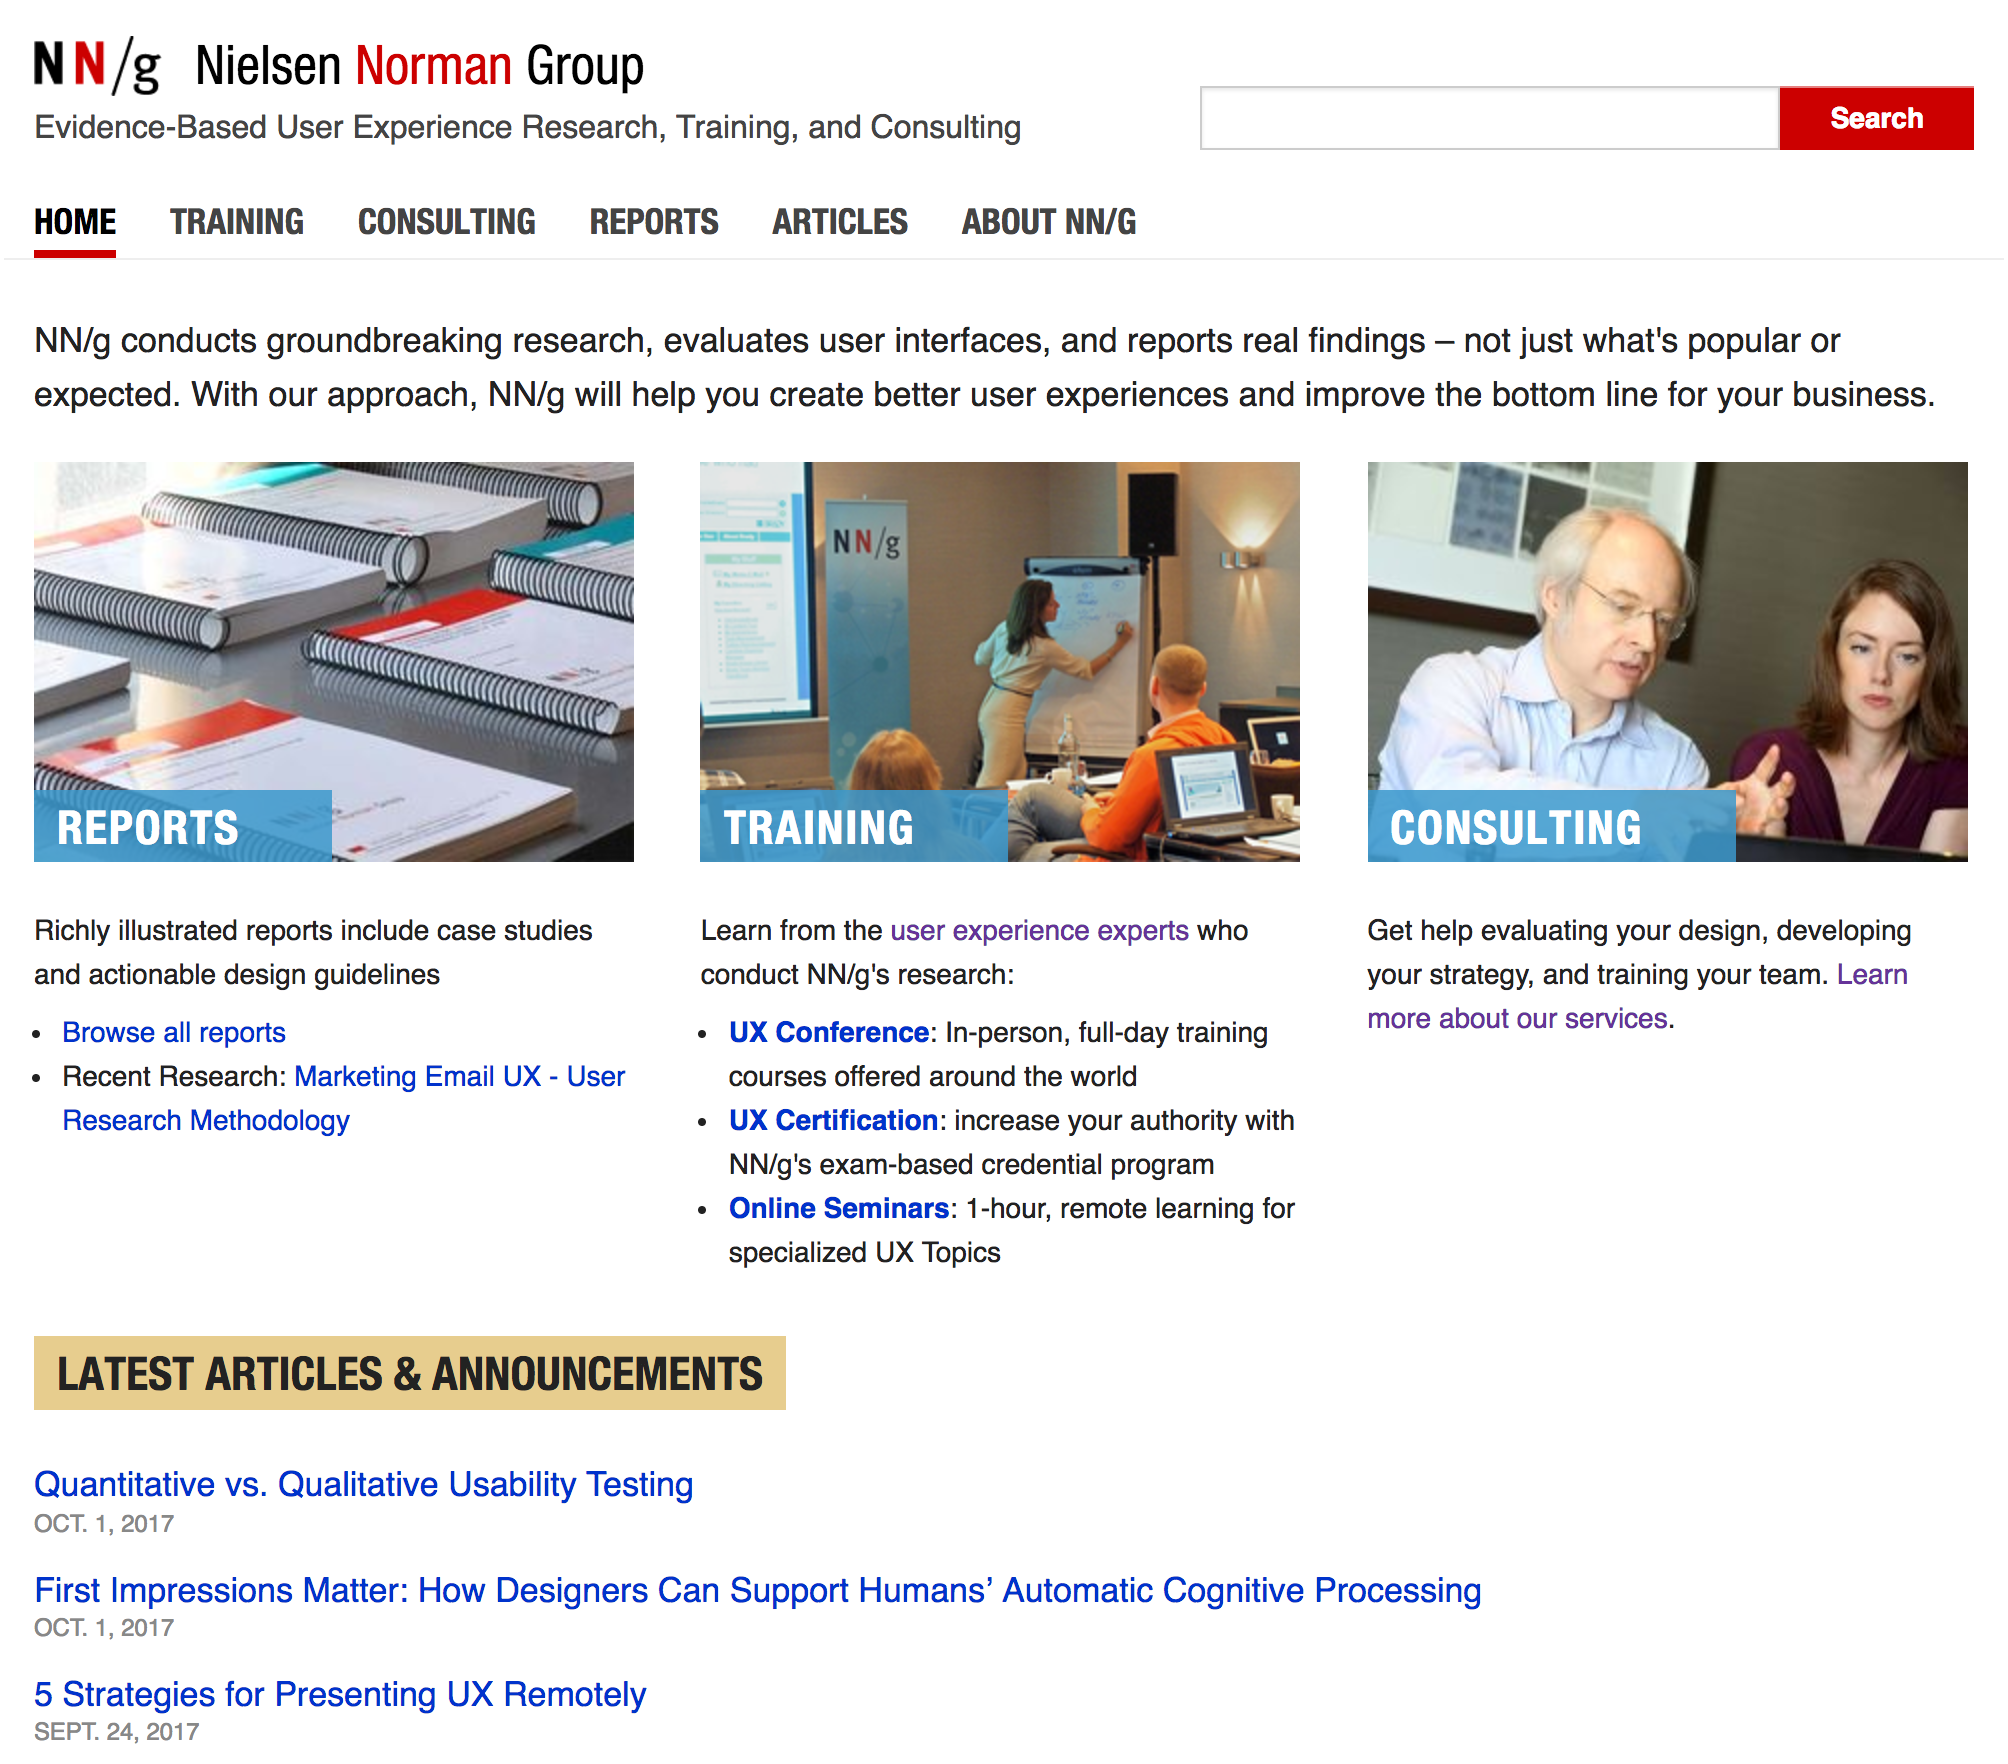
\includegraphics[scale=.2]{assets/nngroup}}
		%\caption{  }
	\end{figure}
\end{frame}

\begin{frame}
	\frametitle{Nielsen Norman Group}
	`Heuristic evaluation involves having a small set of evaluators examine the interface and judge its compliance with recognised usability principles (the "heuristics").' \\~\\
	\href{https://www.nngroup.com/articles/how-to-conduct-a-heuristic-evaluation/}{Link}
\end{frame}

\begin{frame}
	\frametitle{4 Steps}
	
	\begin{enumerate}
		\item Training - Provide expert with the domain specific knowledge needed for a given test scenario
 		\item Experts carry out evaluation \textbf{(two passes minimum)} in isolation of other experts but usually with one or more observers (`experimenter').
		\item Expert assigns a severity rating to each issue found.
		\item Short debrief to discuss the findings with the relevant stakeholders (usually the other experts and the design team).
	\end{enumerate}
\end{frame}

\begin{frame}
	\frametitle{What is tested?}
	\begin{itemize}
		\item The whole product if time allows of the system is not big.
		\item Parts of the whole specific to individual tasks. 
	\end{itemize}
	
	Experts should run through the experiment at least twice. The first pass allows the expert to familiarise themselves with the task. The second pass, should focus on identifying issues. Any further passes are at the observers discretion but are probably not needed. 

\end{frame}

\begin{frame}
	\frametitle{When?}
	
	`Since the evaluators are not using the system as such (to perform a real task), it is possible to perform heuristic evaluation of user interfaces that exist on paper only and have not yet been implemented (Nielsen 1990). This makes heuristic evaluation suited for use early in the usability engineering lifecycle.' \href{https://www.nngroup.com/articles/how-to-conduct-a-heuristic-evaluation/}{(Nielsen, 1995) }
\end{frame}

\begin{frame}

	\huge{How many experts should evaluate an interface?}

\end{frame}

\begin{frame}
	\begin{figure}
		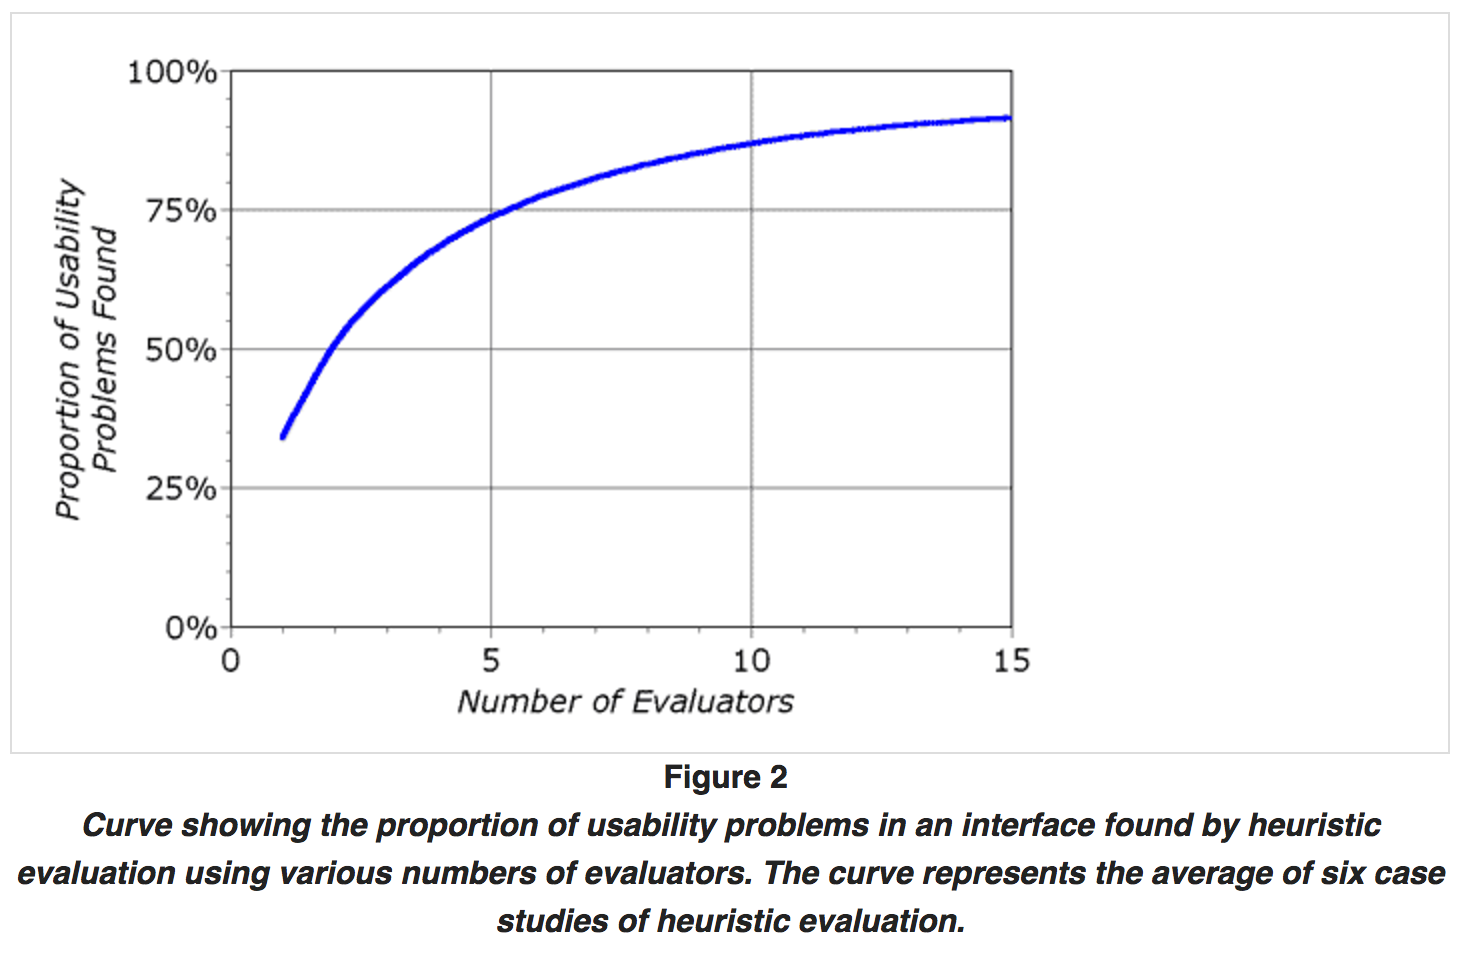
\includegraphics[scale=.4]{assets/num-found}
		%\caption{  }
	\end{figure}
\end{frame}

\begin{frame}
	\begin{figure}
		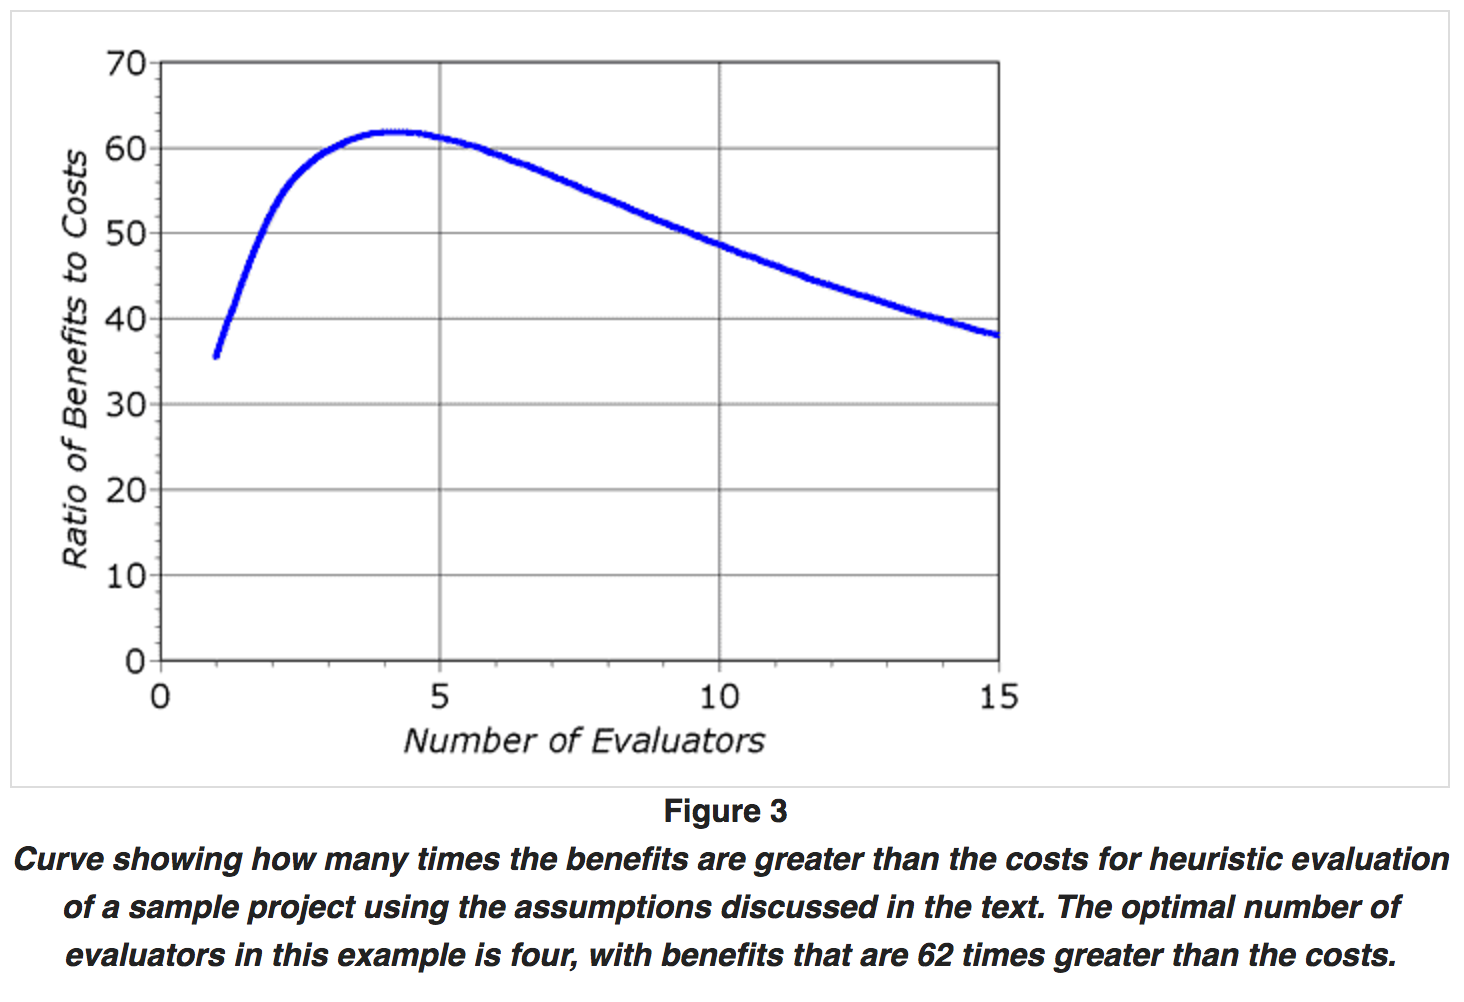
\includegraphics[scale=.4]{assets/costvsben}
		%\caption{  }
	\end{figure}
\end{frame}

\begin{frame}
	\frametitle{What Issues are we Looking for?}
	we are looking for issues in located in a dialogue in four different ways: \\~\\
	
	\begin{enumerate}
		\item at a single location in the interface 
		\item at two or more locations that have to be compared to find the problem
		\item as a problem with the overall structure of the interface, 
		\item and finally as something that ought to be included in the interface but is currently missing. 
	\end{enumerate}
	\href{https://www.nngroup.com/articles/usability-problems-found-by-heuristic-evaluation/}{\tiny{link}}
	
	42\% likely to identify major issues vs. 32\% chance of spotting minor issues (Nielsen 1992).
		
\end{frame}



% --------------------------------------- Nielsen Heuristics 1994

\begin{frame}
	\frametitle{The Heuristics - Nielson 1994}
		
	\begin{itemize}
		\item \textbf{Visibility of system status:} The system should always keep users informed about what is going on, through appropriate feedback within reasonable time.
		\item \textbf{Match between system and the real world:} The system should speak the users' language, with words, phrases and concepts familiar to the user, rather than system-oriented terms. Follow real-world conventions, making information appear in a natural and logical order.
		\item \textbf{User control and freedom:} Users often choose system functions by mistake and will need a clearly marked "emergency exit" to leave the unwanted state without having to go through an extended dialogue. Support undo and redo.
	\end{itemize}
\end{frame}	
		
\begin{frame}		
	\begin{itemize}
		\item \textbf{Consistency and standards:} Users should not have to wonder whether different words, situations, or actions mean the same thing. Follow platform conventions.
		\item \textbf{Error prevention:} Even better than good error messages is a careful design which prevents a problem from occurring in the first place. Either eliminate error-prone conditions or check for them and present users with a confirmation option before they commit to the action.
		\item \textbf{Recognition rather than recall:} Minimize the user's memory load by making objects, actions, and options visible. The user should not have to remember information from one part of the dialogue to another. Instructions for use of the system should be visible or easily retrievable whenever appropriate.
	\end{itemize}	
\end{frame}
					
\begin{frame}		
	\begin{itemize}
		\item \textbf{Flexibility and efficiency of use: } Accelerators?unseen by the novice user?may often speed up the interaction for the expert user such that the system can cater to both inexperienced and experienced users. Allow users to tailor frequent actions.
		\item \textbf{Aesthetic and minimalist design: } Dialogues should not contain information which is irrelevant or rarely needed. Every extra unit of information in a dialogue competes with the relevant units of information and diminishes their relative visibility.
		\item \textbf{Help users recognise, diagnose, and recover from errors: } Error messages should be expressed in plain language (no codes), precisely indicate the problem, and constructively suggest a solution.
	\end{itemize}
\end{frame}		
		
\begin{frame}		
	\begin{itemize}
		\item \textbf{Help and documentation: }Even though it is better if the system can be used without documentation, it may be necessary to provide help and documentation. Any such information should be easy to search, focused on the user's task, list concrete steps to be carried out, and not be too large.
	\end{itemize}
\end{frame}	

\begin{frame}
	\frametitle{Severity ratings}
	`can be used to allocate the most resources to fix the most serious problems and can also provide a rough estimate of the need for additional usability efforts. ' \href{https://www.nngroup.com/articles/how-to-rate-the-severity-of-usability-problems/}{Link}
	
	\begin{enumerate}
		\setcounter{enumi}{0}
		\item I don't agree that this is a usability problem at all 
		\item Cosmetic problem only: need not be fixed unless extra time is available on project 
		\item Minor usability problem: fixing this should be given low priority 
		\item Major usability problem: important to fix, so should be given high priority 
		\item Usability catastrophe: imperative to fix this before product can be released
	\end{enumerate}

\end{frame}

% --------------------------------------- WASTE


\end{document}








